\documentclass[letterpaper, reqno,11pt]{article}
\usepackage[margin=1.0in]{geometry}
\usepackage{color,latexsym,amsmath,amssymb,graphicx,float,listings,tikz}
\usepackage{hyperref}

\hypersetup{
colorlinks=true,
linkcolor=magenta,
filecolor=magenta,
urlcolor=cyan,
}

\graphicspath{ {images/} }

\begin{document}
\pagenumbering{arabic}
\title{MATH318 Homework 4}
\date{09/02/23}
\author{Xander Naumenko}
\maketitle

{\medskip\noindent\bf Question 1a.} The cumulative distribution function is the probability that $T$ is less than a certain value $t$: 
\[
P(T>t)=P(\frac{1}{2}X^2>t)=P(X>\sqrt{2t}) =\begin{cases}
    0&\text{ if }t\leq \frac{9}{2}\\
    \frac{\sqrt{2t}-3}{5} &\text{ if }\frac{9}{2}<t<32\\
    1&\text{ if }t\geq 32\\
\end{cases}
.\]

{\medskip\noindent\bf Question 1b.} The probability density function is the derivative of the $CDF$: 
\[
f(t)=\frac{d}{dt}CDF(t)=\frac{d}{dt}\left( \frac{\sqrt{2t} -3}{5} \right) =\frac{1}{5\sqrt{2t} }
.\]

{\medskip\noindent\bf Question 1c.} Taking the integral: 
\[
    ET=\int_{\frac{9}{2}}^{32} \frac{t}{5\sqrt{2t} }dt = \left( \frac{\sqrt{2}t ^{\frac{3}{2}}}{15}  \right) \bigg|_{\frac{9}{2}}^{32}=16.17
.\]

{\medskip\noindent\bf Question 2a.} Clearly the first coupon will be obtained with probability 1. Once that event has happened, the probability that the next one is unique is $\frac{n-1}{n}$, which is a geometric random variable. This process repeats until all the unique coupons have been picked. The parameter of each random variable is the probability, which for the $i$th coupon is $p=\frac{n+1-i}{n}$. Consider $G(p)$ to be a geometric random variable with parameter p, then
\[
T=\sum_{i=1}^{n}G(\frac{n+1-i}{n})
.\]

{\medskip\noindent\bf Question 2b.} Using the hint: 
\[
    ET=\sum_{i=1}^{n}EG(\frac{n+1-i}{n})=n\sum_{i=1}^{n}\frac{1}{n+1-i}=n\sum_{i=1}^{n}\frac{1}{i}
.\]

{\medskip\noindent\bf Question 3a.} Since $T,B$ are independent their joint PDF is simply $f(t,b)=6e^{-6t}4e^{-4b}= 24 e^{-6t-4b }$

{\medskip\noindent\bf Question 3b.} Taking an integral over the part of the plane where $t<b$: 
\[
p=\int_0^{\infty}\int_0^{b}24e^{-6t-4b}dtdb=\int_0^\infty -4e^{-10b}+4e^{-4b}db=1-\frac{4}{10}=0.6
.\]

{\medskip\noindent\bf Question 3c.} As the hint suggests let $X=\min(T,B)$. Then we have 
\[
P(X>y)=P(T>y)P(B>y)=e^{-6y}e^{-4y}=e^{-10y}
.\]
Taking the distribution to get the PMF: 
\[
f(y)=\frac{d}{dy}P(X<y)=\frac{d}{dy}(1-e^{-10y})=10e^{-10y}
.\]
This is just an exponential distribution with parameter $10$. 

{\medskip\noindent\bf Question 4.} $X,Y$ are independent (since they are both just N(0, 1)), so the joint probability distribution is: 
\[
    P(R)=\left(\frac{1}{\sqrt{2\pi} }e^{-\frac{1}{2}x^2}\right)\left(\frac{1}{\sqrt{2\pi} }e^{-\frac{1}{2}y^2}\right)=\frac{e^{-\frac{1}{2}(x^2+y^2)}}{2\pi}
.\]
To find the cumulative distribution function of $R$ we can integrate over the part of the plane where $X^2+Y^2<R^2$: 
\[
    P(R<r)=\int_0^{r}\int_0^{\sqrt{ r^2-x^2}}\frac{1}{2\pi}e^{-\frac{1}{2}\left( x^2+y^2 \right) }dydx
.\]
\[
    =\frac{1}{2\pi}\int_0^{2\pi}\int_0^{r}e^{-\frac{1}{2}\rho^2}\rho d\rho d\theta=e^{-\frac{1}{2}r^2}
.\]
The probability density is the derivative of the cumulative probability function: 
\[
f(r)=\frac{d}{dr}P(R<r)=re^{-\frac{1}{2}r^2}
.\]
This is called the Rayleigh distribution. 

{\medskip\noindent\bf Question 5a.} Since $X,Y$ are uniform, the probability that $R$ is less than $r$ is just the ratio of the area of the circle of radius less than $r$ to the whole circle. In formula: 
\[
P(R<r)=\frac{\pi r^2}{\pi 1^2}=r^2
.\]
The PDF is just the derivative:
\[
f(r)=\frac{d}{dr} r^2=2r
.\]

{\medskip\noindent\bf Question 5b.} Doing the integral over the possible values: 
\[
ER=\int_0^{1}r 2r dr=\frac{2}{3}r^{3}\bigg|_0^{1}=\frac{2}{3}
.\]

{\medskip\noindent\bf Question 5c.} Since the distribution is uniform, the joint probability distribution of $X$ and $Y$ is $f(x, y)=\frac{1}{\text{area}}=\frac{1}{\pi 1^2}=\frac{1}{\pi}$. For a fixed value of $X=x$, the probability of it occurring can be found by integrating this distribution over $y$: 
\[
f_X(x)=\int_{-\sqrt{1-x^2} }^{\sqrt{1-x^2} }\frac{1}{\pi}dx=\frac{2}{\pi}\sqrt{1-x^2} 
.\]
Since this argument is symmetric between $X$ and $Y$, we have 
\[
f_Y(y)=\frac{2}{\pi}\sqrt{1-y^2}
.\]

{\medskip\noindent\bf Question 5d.} Taking the product of their PDFs: 
\[
f_X(x)f_Y(y)=\frac{4}{\pi}\sqrt{(1-x^2)(1-y^2)}
.\]
Since this does not equal $f(x,y)=\frac{1}{\pi}$, $X$ and $Y$ aren't independent. 

{\medskip\noindent\bf Question 5e.} See figure \ref{fig:5e}. Code: 

\begin{lstlisting}[language=Python]
from random import uniform
import matplotlib.pyplot as plt

n = 10000

pts = [(uniform(-1,1),uniform(-1,1)) for _ in range(n)]
pts_inside = [t for t in pts if t[0]**2 + t[1]**2 < 1]
l = list(zip(*pts_inside))

plt.scatter(l[0], l[1])
plt.plot()
plt.show()
\end{lstlisting}

\begin{figure}[htpb]
    \centering
    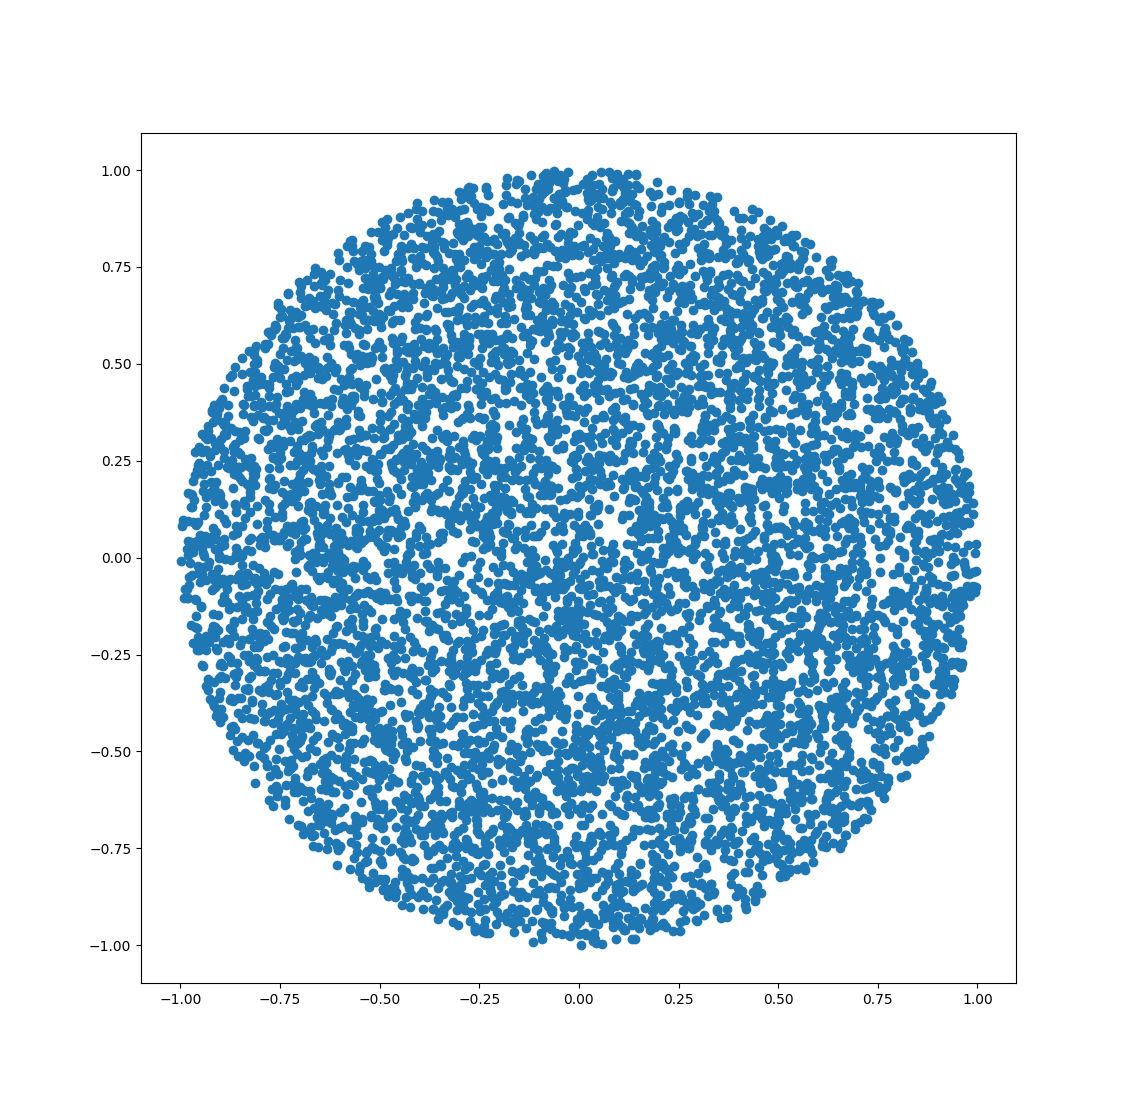
\includegraphics[width=0.8\textwidth]{5e}
    \caption{5e}
    \label{fig:5e}
\end{figure}

{\medskip\noindent\bf Question 5f.} See figure \ref{fig:5f}. The distribution does not appear to be random, as there is a bunching up for this one around 0. This is because the probability distribution function for $R$ is not uniform as we saw in part a. Code: 

\begin{lstlisting}[language=Python]
from random import uniform
import matplotlib.pyplot as plt
import math

n = 10000

rtheta = [(uniform(0,1),uniform(0, 2*math.pi)) for _ in range(n)]
pts = [(r*math.cos(t), r*math.sin(t)) for (r,t) in rtheta]
l = list(zip(*pts))

plt.scatter(l[0], l[1])
plt.plot()
plt.show()
\end{lstlisting}

\begin{figure}[htpb]
    \centering
    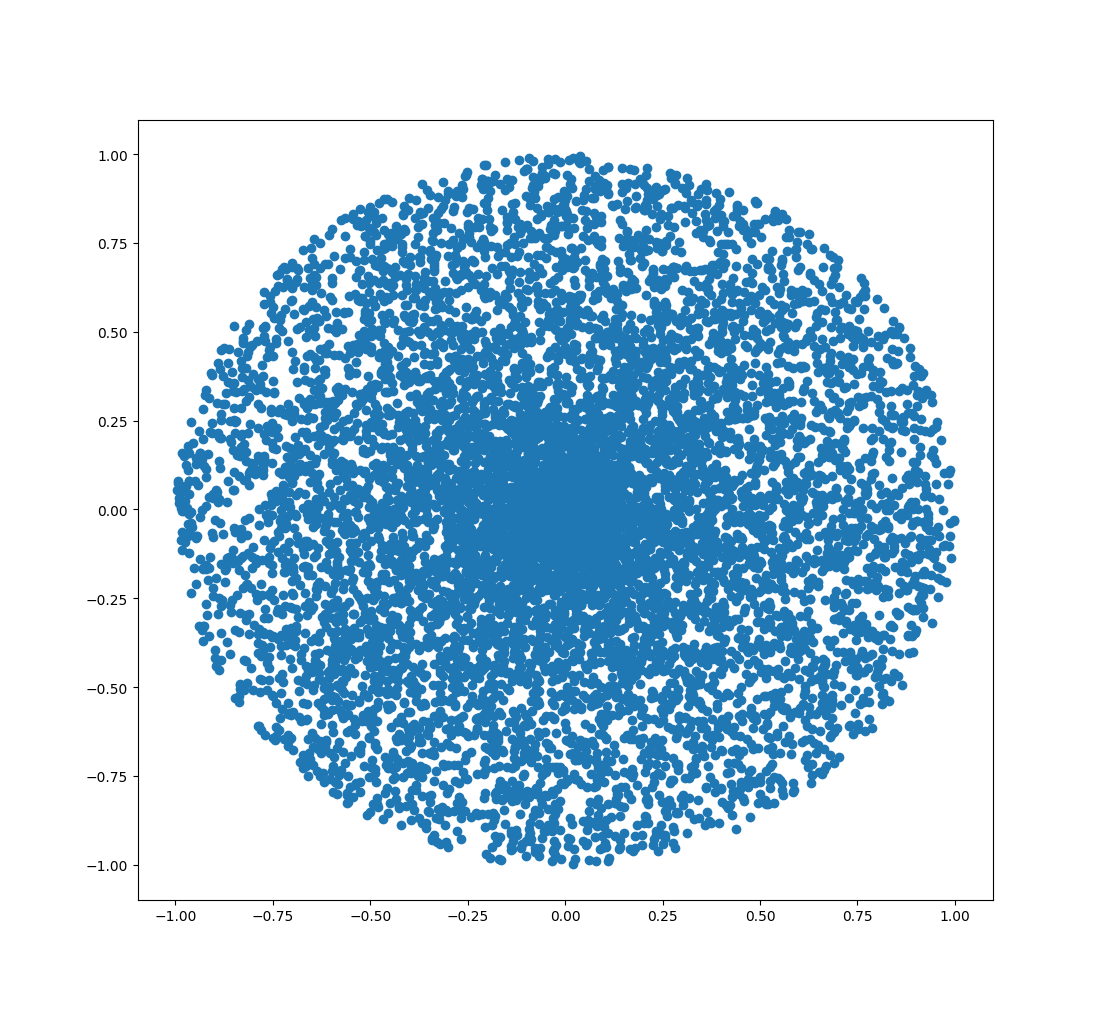
\includegraphics[width=0.8\textwidth]{5f}
    \caption{5f}
    \label{fig:5f}
\end{figure}

{\medskip\noindent\bf Question 5g.} From multivariate calculus, we have that 
\[
\text{area}(A)=\iint_A r drd\theta
.\]
Since this is identical to what we're trying to find except for a factor of $\frac{1}{\pi}$, we have that 
\[
f(r,\theta)=\frac{r}{\pi}
.\]

{\medskip\noindent\bf Question 6a,b,c.} The graphs can be seen in figures \ref{fig:6a}, \ref{fig:6b} and \ref{fig:6c}. The code:

\begin{lstlisting}[language=Python]
import numpy as np
import numpy.random as rn
import matplotlib.pyplot as plt

num = 10000

normals = rn.normal(np.zeros(num))
exps = rn.exponential(np.ones(num)/2)
cauchys = rn.standard_cauchy(num)
for dist in (normals, exps, cauchys):
    averages = []
    s = 0
    ns = np.arange(num)
    for n in ns:
        s += dist[n]
        averages.append(s/(n+1))

    plt.plot(ns, averages)
    plt.show()
\end{lstlisting}

\begin{figure}[htpb]
    \centering
    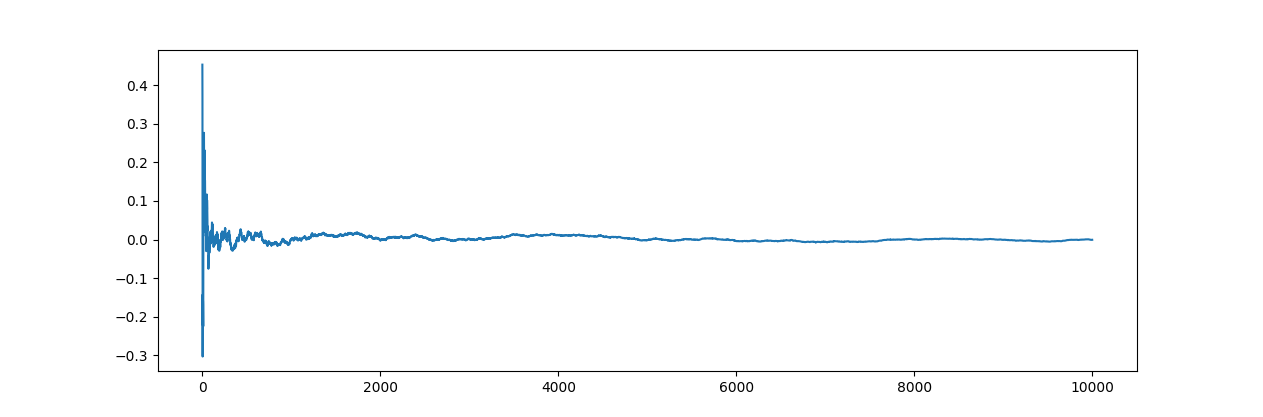
\includegraphics[width=0.8\textwidth]{6a}
    \caption{6a}
    \label{fig:6a}
\end{figure}

\begin{figure}[htpb]
    \centering
    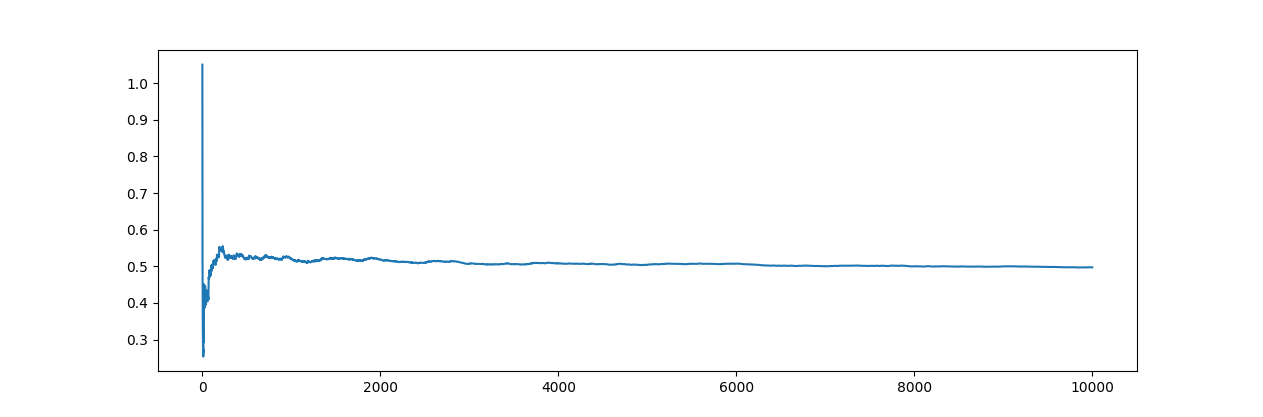
\includegraphics[width=0.8\textwidth]{6b}
    \caption{6b}
    \label{fig:6b}
\end{figure}

\begin{figure}[htpb]
    \centering
    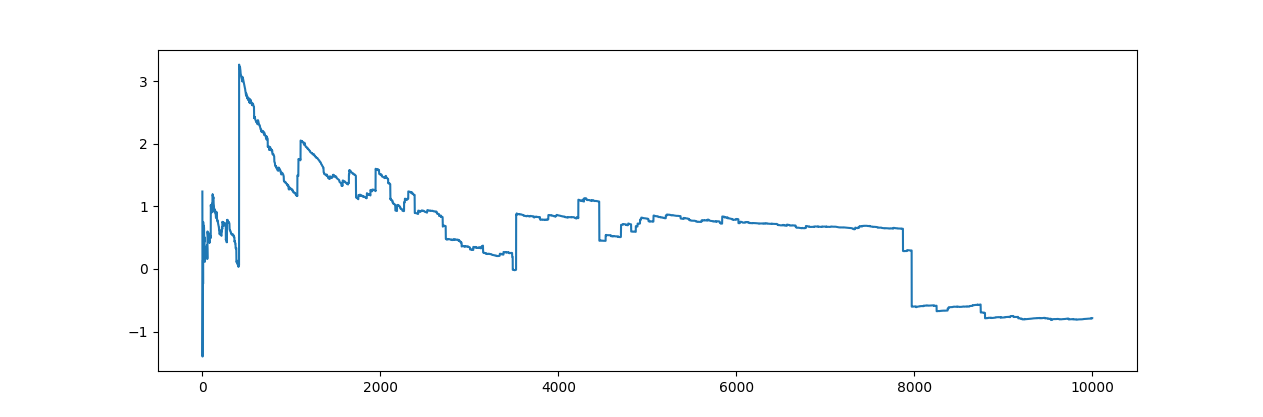
\includegraphics[width=0.8\textwidth]{6c}
    \caption{6c}
    \label{fig:6c}
\end{figure}

{\medskip\noindent\bf Question 6d.} The plot from part a converges to $0$ and the plot from part b converges to $0.5$. These make sense as the mean for the normal and exponential distribution are $0$ and $\frac{1}{\lambda}$ respectively. The plot from part c doesn't seem to converge, and each time the simulation is run the graph seems to change. 

\end{document}
